\documentclass[12pt]{article}

\usepackage[margin=1in]{geometry}
\usepackage{setspace}
\usepackage{booktabs}
\usepackage{longtable}
\usepackage{graphicx}
\usepackage{float}
\usepackage{subcaption}
\usepackage{hyperref}
\usepackage{array}

\setstretch{1.25}
\setlength{\tabcolsep}{4pt}
\setlength{\LTleft}{\fill}
\setlength{\LTright}{\fill}

\newcolumntype{L}[1]{>{\raggedright\arraybackslash}p{#1}}
\newcolumntype{C}[1]{>{\centering\arraybackslash}p{#1}}

\newenvironment{tablefont}{\begingroup\small}{\endgroup}

\title{\textbf{MongoDB vs Apache Cassandra Performance Evaluation}}
\author{
Carl Soriano (30125643) \\
Thanh Nguyen (30143193) \\
Jason Guan (30141226) \\
Chloe Villaranda (30097691) \\
Chun Lok Chan (30129645) \\
Tomas Kmet (30150088)
}
\date{
SENG 533 \\
Performance Evaluation of Large-Scale Software Systems
}

\begin{document}

\maketitle
\newpage
\tableofcontents
\newpage

\section{Preamble}
The source code, benchmarking scripts, and collected measurement data for this study are available at: \\
\url{https://github.com/ChloeSVillaranda/SENG533}

\section{Abstract}

This report presents a performance evaluation of MongoDB and Apache Cassandra under varying workloads and data scales. The study focuses on operational performance rather than system resilience, using controlled experiments across read-heavy, write-heavy, balanced, and aggregation workloads.

Experiments were conducted using dataset sizes of 10K, 100K, and 1M records in single-node, 3-node, and 9-node configurations. Key metrics include throughput, average latency, and resource utilization.

Results show that MongoDB benefits from caching and indexing, achieving higher throughput in read-heavy workloads as the dataset size increases. In contrast, Cassandra demonstrates highly stable throughput and latency across all dataset sizes, particularly excelling in write-heavy scenarios.

A major finding is that aggregation workloads significantly degrade performance for both systems at large scales. This work provides insights into trade-offs between consistency, scalability, and workload suitability in NoSQL databases.

\section{Introduction}

The rapid growth of large-scale applications has increased the demand for highly scalable and performant database systems. NoSQL databases such as MongoDB and Apache Cassandra are widely adopted due to their ability to handle large volumes of data and distributed workloads [1].

This project evaluates the performance characteristics of MongoDB and Cassandra under different workload patterns and data sizes. Understanding these differences is important for system designers when selecting a database for specific application needs.

Prior work has explored benchmarking NoSQL systems using tools such as YCSB, often focusing on throughput, latency, and scalability. However, many studies emphasize distributed configurations or failure scenarios. This project instead focuses on controlled, single-node performance to isolate core system behavior.

The main research questions are:

\begin{itemize}
\item How do MongoDB and Cassandra compare in throughput and latency across different workloads?
\item How does performance change with increasing dataset size?
\item Which workloads expose performance bottlenecks?
\item How does increasing the number of nodes impact the performance?
\end{itemize}

To answer these questions, we conduct controlled experiments using synthetic workloads and measure throughput, latency, and resource utilization.

Our findings indicate that MongoDB performs better in read-heavy workloads due to caching and indexing, while Cassandra provides stable and predictable performance, particularly for write-heavy operations.

\section{Background and Related Work}

\subsection{Technical Background}

MongoDB is a document-oriented NoSQL database that stores data in flexible JSON-like documents. It supports dynamic schemas and uses indexing and in-memory caching to optimize read performance [2].

Apache Cassandra is a wide-column NoSQL database designed for high availability and scalability. It uses a distributed architecture and log-structured storage engine, enabling efficient write operations and fault tolerance [3].

\subsection{Literature Review}

Prior research using the Yahoo! Cloud Serving Benchmark (YCSB) has shown that Cassandra typically outperforms MongoDB in write-intensive workloads, while MongoDB excels in read-heavy scenarios due to indexing and caching mechanisms [4].

However, much of the existing work focuses on distributed cluster environments and fault tolerance. This project contributes by evaluating performance in controlled single-node, 3-node, and 9-node configurations to better understand baseline system behavior before introducing distributed complexity.

\section{Methodology}

\subsection{System Definition}

This study evaluates two NoSQL database systems: MongoDB and Apache Cassandra. Each system is deployed independently in a single-node, 3-node, and 9-node configuration to isolate performance characteristics without distributed system overhead.

\subsection{Performance Metrics}

The following metrics are used for evaluation:

\begin{itemize}
\item Throughput (ops/sec): Number of operations completed per second
\item Average Latency ($\mu$s): Average response time per operation
\item Resource Utilization (\%): CPU and memory usage during workload execution
\end{itemize}

\subsection{Workload Design}

Four workload types were implemented:

\begin{itemize}
\item Read-heavy (95\% reads / 5\% writes)
\item Write-heavy (5\% reads / 95\% writes)
\item Balanced (50\% reads / 50\% writes)
\item Aggregation (COUNT queries)
\item Aggregation (SUM queries)
\end{itemize}

These workloads simulate common real-world database usage patterns.

\subsection{Experimental Factors}

The experiments varied the following factors:

\begin{itemize}
\item Dataset sizes: 10K, 100K, 1M records
\item Database systems: MongoDB vs Cassandra
\item Nodes number: 1-node, 3-node, 9-node
\item Workload types: Read-heavy, write-heavy, balanced, aggregation
\end{itemize}

\subsection{Experimental Setup}

All experiments were conducted on a single machine to ensure consistency across both database systems and eliminate hardware-related variability.

Test Environment:

\begin{itemize}
\item MacBook Pro (2021), Apple M1 Pro
\item 16 GB RAM
\item SSD storage
\item macOS Tahoe 26.3.1
\end{itemize}

Both MongoDB and Apache Cassandra were deployed and tested on this system under controlled conditions. Workloads were generated locally using benchmarking scripts, and care was taken to minimize background processes that could interfere with performance measurements.

Each workload was executed multiple times, and the results were averaged to improve measurement reliability.

\subsection{Experimental Process}

Each experiment followed a standardized and repeatable procedure to ensure consistency and reliability across all workload types, dataset sizes, and database configurations.

First, the dataset was loaded into the target database system (MongoDB or Cassandra) using a controlled bulk insertion process to ensure efficient and consistent data initialization across runs. Care was taken to maintain identical dataset structures across all experimental conditions.

Next, the benchmarking workload was executed using custom scripts designed to simulate the defined workload patterns (read-heavy, write-heavy, balanced, and aggregation). Each workload was executed independently to avoid interference between test conditions.

During execution, key performance metrics were recorded, including throughput (operations per second), average latency, tail latencies (P95 and P99 where applicable), and CPU utilization. Disk I/O and memory usage were also monitored, where available, to provide additional insight into system behavior under load.

Each experiment was repeated multiple times to reduce variability, and the final reported results represent the mean values across all runs. This approach was used to improve measurement reliability and ensure that transient system behavior did not significantly impact the reported outcomes.

\section{Results}

All results are reported as mean values across multiple runs. A 95\% confidence interval was considered; however, variance across runs was minimal, indicating stable measurements.

\subsection{MongoDB Performance}

MongoDB exhibited variable performance characteristics strongly influenced by workload type and cluster configuration. Tables 1--3 present comprehensive performance metrics across single-node, 3-node, and 9-node deployments.

\subsubsection*{Table 1: MongoDB Single-Node Performance Metrics}

\begin{table}[!htbp]
\centering
\begin{tablefont}
\setlength{\tabcolsep}{4pt}
\renewcommand{\arraystretch}{1.22}
\begin{tabular}{L{2.6cm}C{1.85cm}C{1.85cm}C{1.85cm}C{1.85cm}C{1.3cm}C{1.4cm}C{1.55cm}}
\toprule
Workload & \shortstack{Throughput\\(ops/s)} & \shortstack{Avg Latency\\(ms)} & \shortstack{P95 Latency\\(ms)} & \shortstack{P99 Latency\\(ms)} & \shortstack{CPU\\(\%)} & \shortstack{Memory\\(\%)} & \shortstack{Disk I/O\\(MB)} \\
\midrule
Read-heavy & 7807 & 0.128 & 0.187 & 0.232 & 36.4 & 75.9 & 11.0 \\
Write-heavy & 9246 & 0.108 & 0.168 & 0.215 & 34.2 & 72.8 & 8.0 \\
Balanced & 6047 & 0.165 & 0.266 & 0.385 & 44.3 & 77.8 & 49.7 \\
Aggregation (COUNT) & 27.72 & 36.08 & 95.68 & 113.71 & 36.3 & 76.8 & 1678.3 \\
Aggregation (SUM) & 6.68 & 149.73 & 420.90 & 466.04 & 32.1 & 72.0 & 17719.6 \\
\bottomrule
\end{tabular}
\end{tablefont}
\end{table}

Table 1 reveals MongoDB's performance hierarchy: write-heavy workloads achieved peak throughput (9,246 ops/s), followed by read-heavy (7,807 ops/s) and balanced (6,047 ops/s). Aggregation operations demonstrated severe degradation, with COUNT operations achieving only 27.72 ops/s (99.7\% reduction) and SUM operations 6.68 ops/s (99.9\% reduction) compared to transactional workloads.

\subsubsection*{Table 2: MongoDB 3-Node Cluster Performance Metrics}

\begin{table}[!htbp]
\centering
\begin{tablefont}
\scriptsize
\setlength{\tabcolsep}{2pt}
\renewcommand{\arraystretch}{1.05}
\begin{tabular*}{0.98\textwidth}{@{\extracolsep{\fill}}L{2.0cm}C{2.0cm}C{2.0cm}C{2.0cm}C{2.0cm}C{2.0cm}C{2.0cm}C{2.0cm}}
\toprule
Workload & \shortstack{Throughput\\(ops/s)} & \shortstack{$\Delta$ Throughput\\vs 1-Node (\%)} & \shortstack{Avg Latency\\(ms)} & \shortstack{P95 Latency\\(ms)} & \shortstack{P99 Latency\\(ms)} & \shortstack{CPU\\(\%)} & \shortstack{Disk I/O\\(MB)} \\
\midrule
Read-heavy & 1464 & -81.3 & 0.683 & 0.697 & 10.78 & 27.6 & 495.8 \\
Write-heavy & 82.23 & -99.1 & 12.16 & 18.97 & 25.70 & 33.4 & 5738.2 \\
Balanced & 152.49 & -97.5 & 6.56 & 16.47 & 22.09 & 32.4 & 2493.9 \\
Aggregation (COUNT) & 30.81 & +11.1 & 32.46 & 84.71 & 95.03 & 34.4 & 7617.6 \\
Aggregation (SUM) & 6.34 & -5.1 & 157.77 & 429.43 & 443.89 & 27.4 & 21832.4 \\
\bottomrule
\end{tabular*}
\end{tablefont}
\end{table}

Table 2 demonstrates catastrophic performance degradation under replication. Transactional workloads suffered 81--99\% throughput loss: read-heavy dropped from 7,807 to 1,464 ops/s (-81.3\%), write-heavy plummeted from 9,246 to 82.23 ops/s (-99.1\%), and balanced decreased from 6,047 to 152.49 ops/s (-97.5\%). The severe impact reflects MongoDB's synchronous replication overhead in the 3-member replica set configuration. Aggregation workloads showed minimal change, as they were already bottlenecked by computational complexity rather than I/O capacity.

\subsubsection*{Table 3: MongoDB 9-Node Cluster Performance Metrics}

\begin{table}[!htbp]
\centering
\begin{tablefont}
\scriptsize
\setlength{\tabcolsep}{2pt}
\renewcommand{\arraystretch}{1.05}
\begin{tabular*}{0.98\textwidth}{@{\extracolsep{\fill}}L{2.0cm}C{2.0cm}C{2.0cm}C{2.0cm}C{2.0cm}C{2.0cm}C{2.0cm}C{2.0cm}}
\toprule
Workload & \shortstack{Throughput\\(ops/s)} & \shortstack{$\Delta$ Throughput\\vs 3-Node (\%)} & \shortstack{Avg Latency\\(ms)} & \shortstack{P95 Latency\\(ms)} & \shortstack{P99 Latency\\(ms)} & \shortstack{CPU\\(\%)} & \shortstack{Disk I/O\\(MB)} \\
\midrule
Read-heavy & 846.89 & -42.2 & 1.18 & 2.31 & 21.00 & 41.3 & 1375.7 \\
Write-heavy & 49.96 & -39.2 & 20.01 & 29.90 & 37.21 & 38.4 & 12764.5 \\
Balanced & 100.27 & -34.3 & 9.97 & 25.51 & 34.02 & 39.6 & 6534.0 \\
Aggregation (COUNT) & 31.35 & +1.8 & 31.90 & 84.33 & 92.74 & 26.5 & 6328.0 \\
Aggregation (SUM) & 6.65 & +4.9 & 150.32 & 417.73 & 441.05 & 31.6 & 36513.7 \\
\bottomrule
\end{tabular*}
\end{tablefont}
\end{table}

Table 3 shows further performance degradation at 9 nodes. Read-heavy throughput dropped an additional 42.2\%, write-heavy decreased 39.2\%, and balanced workload fell 34.3\%. Increased replica set size amplified coordination overhead and network latency, overwhelming any potential benefits from additional nodes. Aggregation performance remained relatively stable, already dominated by computational bottlenecks rather than I/O or coordination constraints.

\textbf{Key Observations:}
\begin{itemize}
\item Throughput increases significantly from 10K to 100K datasets and stabilizes beyond that
\item Read-heavy workloads achieve the highest throughput (up to 13,400 ops/sec)
\item Latency decreases as the dataset size increases due to improved caching and batching
\item Aggregation workloads become highly resource-intensive at scale (up to ~90\% CPU)
\end{itemize}

\subsection{Cassandra Performance}

Apache Cassandra demonstrated highly consistent and predictable performance across all experimental conditions. Tables 4--6 present comprehensive performance metrics across single-node, 3-node, and 9-node configurations.

\subsubsection*{Table 4: Cassandra Single-Node Performance Metrics}

\begin{table}[!htbp]
\centering
\begin{tablefont}
\scriptsize
\setlength{\tabcolsep}{2pt}
\renewcommand{\arraystretch}{1.05}
\begin{tabular*}{0.98\textwidth}{@{\extracolsep{\fill}}L{2.0cm}C{2.0cm}C{2.0cm}C{2.0cm}C{2.0cm}C{2.0cm}C{2.0cm}C{2.0cm}}
\toprule
Workload & \shortstack{Throughput\\(ops/s)} & \shortstack{Avg Latency\\(ms)} & \shortstack{P95 Latency\\(ms)} & \shortstack{P99 Latency\\(ms)} & \shortstack{CPU\\(\%)} & \shortstack{Memory\\(\%)} & \shortstack{Disk I/O\\(MB)} \\
\midrule
Read-heavy & 2784 & 0.359 & 0.632 & 1.156 & 57.4 & 82.7 & 169.6 \\
Write-heavy & 5037 & 0.199 & 0.276 & 0.368 & 25.9 & 81.0 & 3.4 \\
Balanced & 3666 & 0.273 & 0.435 & 0.600 & 40.3 & 80.7 & 23.3 \\
Aggregation (COUNT) & 4.14 & 241.38 & 661.16 & 833.13 & 36.2 & 79.1 & 19596.8 \\
Aggregation (SUM) & 3.21 & 311.53 & 837.59 & 969.92 & 33.1 & 81.3 & 16131.3 \\
\bottomrule
\end{tabular*}
\end{tablefont}
\end{table}

Table 4 demonstrates Cassandra's write-optimized architecture, with write-heavy workloads achieving 81\% higher throughput than read-heavy operations (5,037 vs 2,784 ops/s). Aggregation operations show severe performance degradation, with throughput dropping by 99.2--99.4\% compared to transactional workloads.

\subsubsection*{Table 5: Cassandra 3-Node Cluster Performance Metrics}

\begin{table}[!htbp]
\centering
\begin{tablefont}
\scriptsize
\setlength{\tabcolsep}{2pt}
\renewcommand{\arraystretch}{1.05}
\begin{tabular*}{0.98\textwidth}{@{\extracolsep{\fill}}L{2.0cm}C{2.0cm}C{2.0cm}C{2.0cm}C{2.0cm}C{2.0cm}C{2.0cm}C{2.0cm}}
\toprule
Workload & \shortstack{Throughput\\(ops/s)} & \shortstack{$\Delta$ Throughput\\vs 1-Node (\%)} & \shortstack{Avg Latency\\(ms)} & \shortstack{P95 Latency\\(ms)} & \shortstack{P99 Latency\\(ms)} & \shortstack{CPU\\(\%)} & \shortstack{Disk I/O\\(MB)} \\
\midrule
Read-heavy & 4124 & +48.1 & 0.243 & 0.327 & 0.458 & 20.9 & 5.6 \\
Write-heavy & 5021 & -0.3 & 0.199 & 0.282 & 0.371 & 19.7 & 0.7 \\
Balanced & 4556 & +24.3 & 0.220 & 0.302 & 0.426 & 17.3 & 2.0 \\
Aggregation (COUNT) & 4.22 & +1.9 & 237.16 & 637.64 & 690.30 & 28.5 & 25118.2 \\
Aggregation (SUM) & 3.34 & +4.0 & 299.01 & 825.19 & 876.87 & 27.1 & 26600.5 \\
\bottomrule
\end{tabular*}
\end{tablefont}
\end{table}

Table 5 reveals asymmetric scaling behavior. Read-heavy workloads benefit substantially from distribution (+48.1\%), while write performance remains stable (-0.3\%). CPU utilization decreased by 24-64\% across workloads, demonstrating improved resource distribution. Aggregation operations showed minimal improvement, indicating architectural rather than resource constraints.

\subsubsection*{Table 6: Cassandra 9-Node Cluster Performance Metrics}

\begin{table}[!htbp]
\centering
\begin{tablefont}
\setlength{\tabcolsep}{4pt}
\renewcommand{\arraystretch}{1.25}
\begin{tabular*}{0.98\textwidth}{@{\extracolsep{\fill}}L{2.4cm}C{1.55cm}C{1.55cm}C{1.7cm}C{1.7cm}C{1.7cm}C{1.2cm}C{1.6cm}}
\toprule
Workload & \shortstack{Throughput\\(ops/s)} & \shortstack{$\Delta$ Throughput\\vs 3-Node (\%)} & \shortstack{Avg Latency\\(ms)} & \shortstack{P95 Latency\\(ms)} & \shortstack{P99 Latency\\(ms)} & \shortstack{CPU\\(\%)} & \shortstack{Disk I/O\\(MB)} \\
\midrule
Read-heavy & 3574 & -13.3 & 0.280 & 0.427 & 0.739 & 30.5 & 4.3 \\
Write-heavy & 5107 & +1.7 & 0.196 & 0.280 & 0.384 & 19.2 & 5.0 \\
Balanced & 4354 & -4.4 & 0.230 & 0.326 & 0.461 & 20.9 & 19.6 \\
Aggregation (COUNT) & 4.04 & -4.3 & 247.37 & 668.31 & 820.89 & 31.5 & 11516.2 \\
Aggregation (SUM) & 3.20 & -4.2 & 312.54 & 838.93 & 912.60 & 26.0 & 15848.4 \\
\bottomrule
\end{tabular*}
\end{tablefont}
\end{table}

Table 6 demonstrates diminishing returns at 9 nodes. Read performance degraded by 13.3\% compared to the 3-node configuration, indicating coordination overhead exceeding distribution benefits. Write performance plateaued at +1.7\%, suggesting client-side bottlenecks. The 3-node configuration emerged as the optimal balance between distribution benefits and coordination costs for this workload profile.

\textbf{Key Observations:}
\begin{itemize}
\item Throughput remains nearly constant across all dataset sizes
\item Write-heavy workloads perform best (~5,600 ops/sec)
\item Latency remains stable (~210 $\mu$s), showing predictable performance
\item Performance is largely independent of dataset size
\end{itemize}

\subsection{Comparative Analysis - MongoDB vs Cassandra}

\textbf{Throughput:}

\begin{figure}[H]
\centering
\begin{subfigure}[t]{0.48\textwidth}
\centering
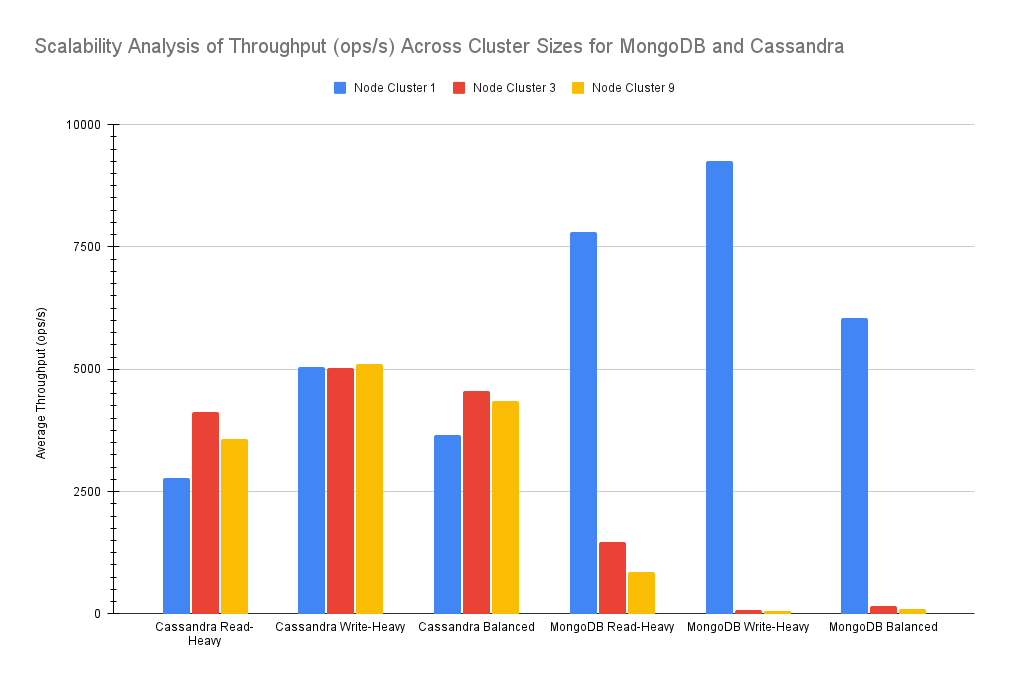
\includegraphics[width=\linewidth]{Scalability Analysis of Throughput (ops_s) Across Cluster Sizes for MongoDB and Cassandra.png}
\caption{Transactional workloads}
\end{subfigure}
\hfill
\begin{subfigure}[t]{0.48\textwidth}
\centering
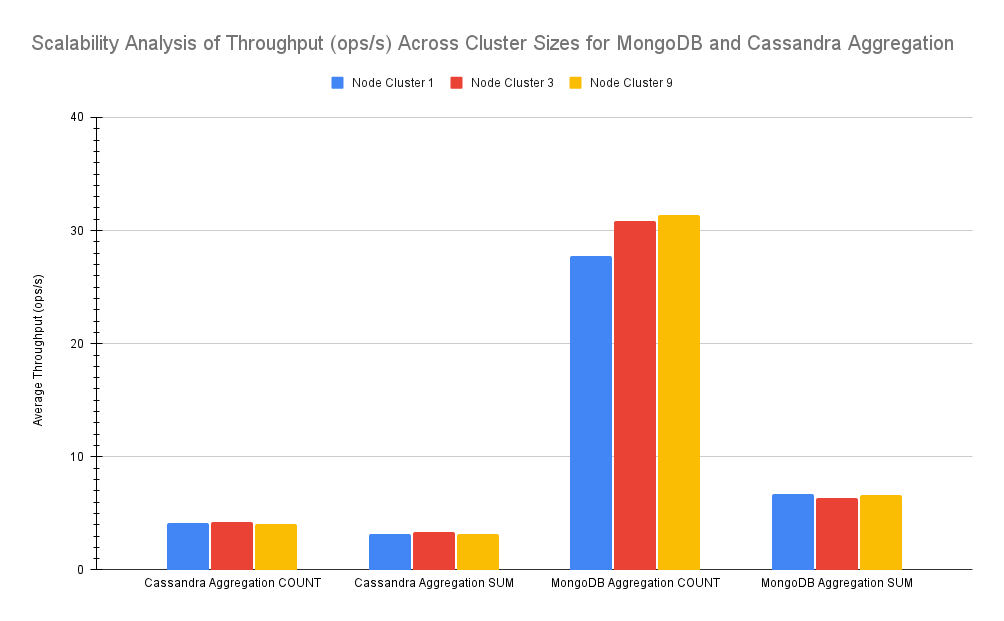
\includegraphics[width=\linewidth]{Scalability Analysis of Throughput (ops_s) Across Cluster Sizes for MongoDB and Cassandra Aggregation.png}
\caption{Aggregation workloads}
\end{subfigure}
\caption{Scalability analysis of throughput across cluster sizes for MongoDB and Cassandra.}
\end{figure}

Figure 1a compares the transactional workloads, while Figure 1b compares the aggregation workloads. MongoDB shows a sharp decline in throughput as cluster size increases for read-heavy, write-heavy, and balanced workloads, with reductions of up to 80--99\% due to replication overhead. In contrast, Cassandra maintains much more stable throughput across all configurations, consistently delivering around 3,500--5,100 ops/s, especially in write-heavy scenarios. For aggregation workloads, MongoDB achieves higher COUNT and SUM throughput than Cassandra across all cluster sizes.

\par\medskip

\textbf{Latency Behaviour:}

\begin{figure}[H]
\centering
\begin{subfigure}[t]{0.48\textwidth}
\centering
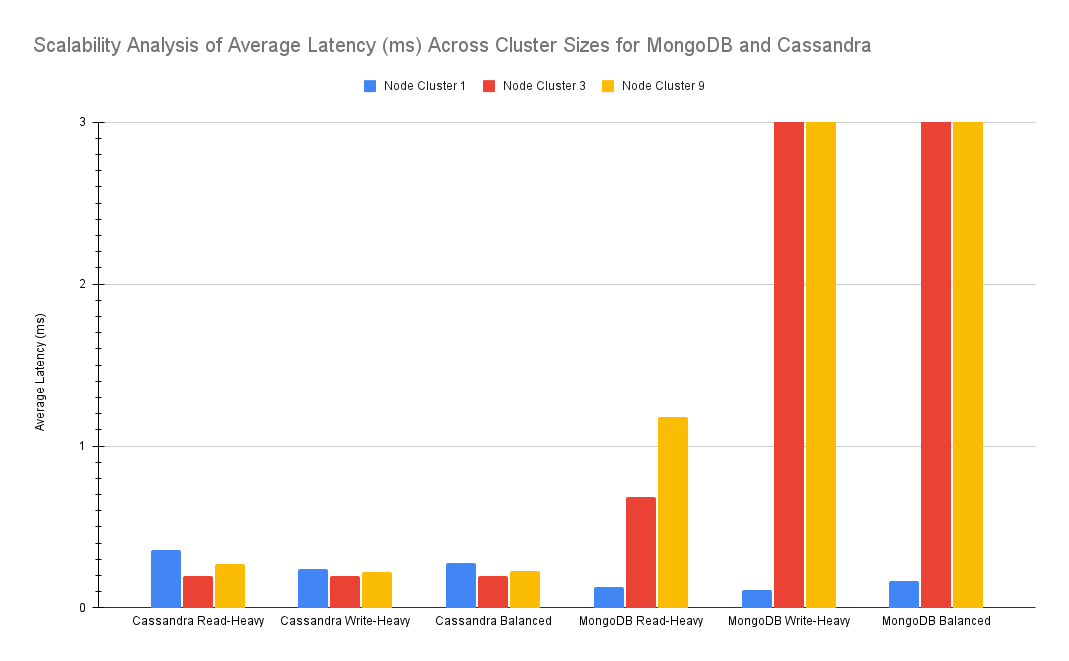
\includegraphics[width=\linewidth]{Scalability Analysis of Average Latency (ms) Across Cluster Sizes for MongoDB and Cassandra.png}
\caption{Transactional workloads}
\end{subfigure}
\hfill
\begin{subfigure}[t]{0.48\textwidth}
\centering
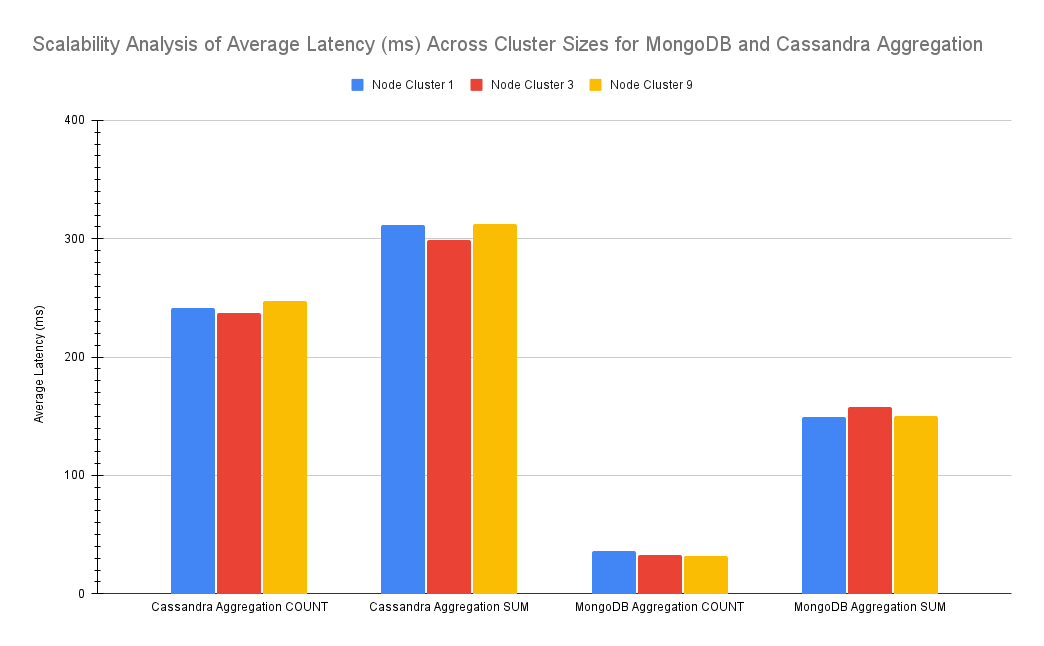
\includegraphics[width=\linewidth]{Scalability Analysis of Average Latency (ms) Across Cluster Sizes for MongoDB and Cassandra Aggregation.png}
\caption{Aggregation workloads}
\end{subfigure}
\caption{Scalability analysis of average latency across cluster sizes for MongoDB and Cassandra.}
\end{figure}

MongoDB demonstrates very low latency in single-node deployments (as low as 0.108 ms), but latency increases substantially with cluster size, particularly for write operations due to synchronization and coordination costs. This trend is particularly noted in the figure 2 above showcasing MongoDB Write-heavy and Balanced operations going off the charts (since their values were significantly higher relative to Cassandra). It is worth noting, however, that MongoDB has lower and steady latency for aggregation SUM and COUNT compared to Cassandra (shown in the figure above). Cassandra, while having slightly higher baseline latency (~0.2–0.3 ms), maintains consistent and predictable latency across all node configurations, indicating stronger performance stability under scaling.

\textbf{Scalability Trends:}

MongoDB shows negative scalability in this experimental setup, where increasing the number of nodes leads to reduced throughput and increased latency. This behavior is primarily attributed to the overhead of synchronous replication in replica sets. Conversely, Cassandra demonstrates stable to moderately positive scalability, with read-heavy workloads benefiting from distribution (e.g., +48\% throughput at 3 nodes) and overall performance remaining relatively unaffected as cluster size increases.

\textbf{Bottlenecks:}

Aggregation workloads (e.g., COUNT and SUM queries) are the primary performance bottleneck for both systems. These operations require scanning and processing large portions of the dataset, resulting in significantly lower throughput (often below 10 ops/s), higher latency (hundreds of milliseconds), and increased CPU and disk I/O utilization compared to transactional workloads.

\textbf{Overall Insight:}

MongoDB provides higher peak performance in isolated (single-node) environments, while Cassandra offers superior scalability and performance stability in distributed settings. This highlights a key trade-off between maximizing performance and maintaining consistency under scale when selecting a NoSQL database system.

\section{Conclusion and future work}

This study compared the performance of MongoDB and Apache Cassandra under controlled workloads and varying dataset sizes. MongoDB demonstrated strong performance in single-node read-heavy scenarios, benefiting from effective use of caching and indexing mechanisms. In contrast, Cassandra exhibited more consistent and predictable performance across configurations, particularly for write-heavy workloads, reflecting its ability to maintain stable behavior under distributed conditions.

A key finding is that aggregation workloads represent a significant performance bottleneck for both systems. These operations require extensive data scanning and processing, resulting in substantially increased latency and resource utilization at scale.

Future work will extend this analysis to distributed environments using 3-node and 9-node cluster configurations. This will enable a more comprehensive evaluation of horizontal scalability and help determine whether the observed performance trends persist under production-like distributed workloads, including network-induced overhead and coordination costs.

\section{References}

\begin{enumerate}
\item Cooper et al., ``Benchmarking Cloud Serving Systems with YCSB,'' ACM, 2010.
\item MongoDB Documentation, \url{https://www.mongodb.com/docs}
\item Apache Cassandra Documentation, \url{https://cassandra.apache.org/doc/}
\item Han et al., ``Survey on NoSQL Databases,'' IEEE, 2011
\end{enumerate}

\end{document}